
\par{Listing \ref{private_local_memory_kernel} shows the kernel that uses together private and local memory to cache column B.}

\lstinputlisting[float,caption={Kernel making use of \emph{private memory} and \emph{local memory}.},label={private_local_memory_kernel}, 
                style=customc]{/Users/clalanne/GitHubProjects/OpenCLNotes/src/code/private_local_memory.c}

\par{The results can be seen in figure \ref{RowsCols}}

\begin{figure}[!h]
    \centering
    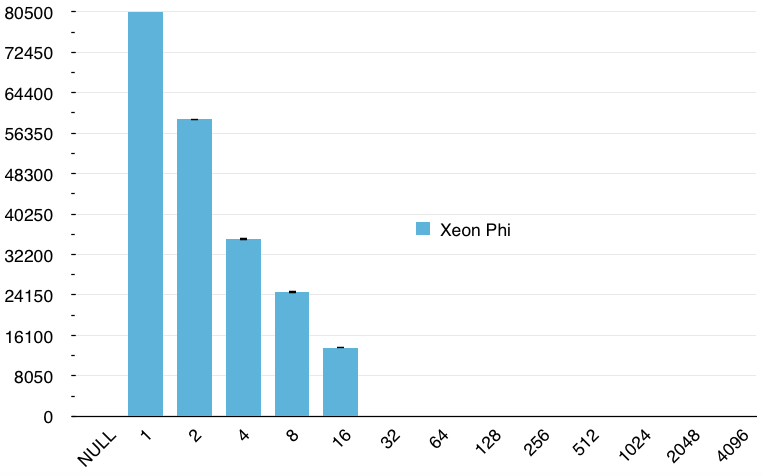
\includegraphics[width=0.49\textwidth]{figures/opt3_phi.png}
    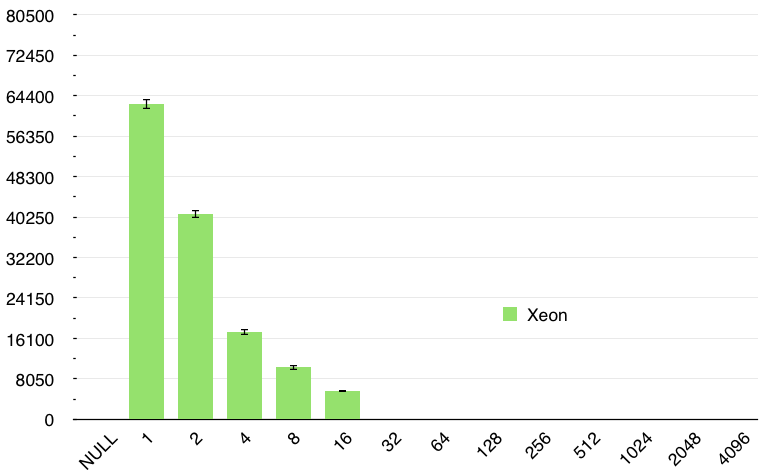
\includegraphics[width=0.49\textwidth]{figures/opt3_cpu.png}
    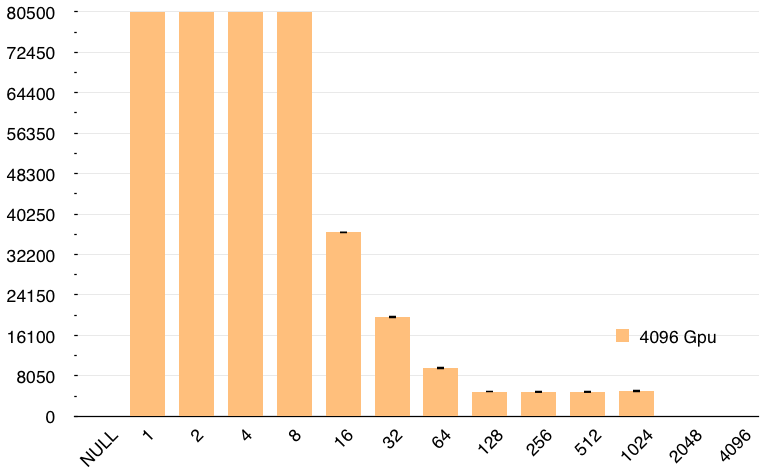
\includegraphics[width=0.49\textwidth]{figures/opt3_gpu.png}
    \caption{Rows and columns optimisation matrix multiplication in different architectures.}
    \label{RowsCols}
\end{figure}

\par{\ref{RowsColsComp}}

\begin{figure}[!h]
    \centering
    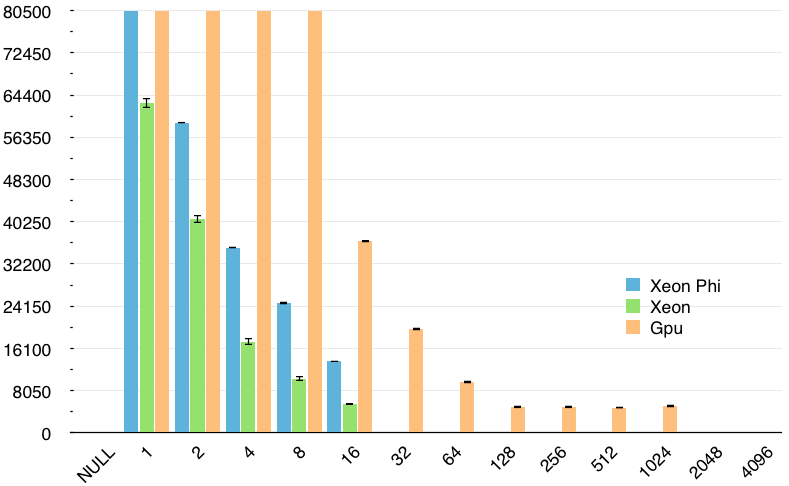
\includegraphics[width=0.6\textwidth]{figures/opt3_comp.png}
    \caption{Rows and columns optimisation matrix multiplication with more work in different architectures comparison.}
    \label{RowsColsComp}
\end{figure}

